\subsection{Service-Oriented Component Model}

\begin{frame}{iPOJO: A SOCM in Java}
\begin{block}{iPOJO Concepts}
\begin{tabular}{lp{.7\textwidth}}
Component & Instance of a \textit{Factory} class\\
\hline
Factory & (Annotated) Java class, modified by iPOJO after compilation\\
\hline
Handler & Manages a component according to information in its Factory\\
\end{tabular}
\end{block}

\begin{block}{Features}
\begin{itemize}
\item Components are bound by services
\item All the binding and life-cycle management is done by handlers
\item The Factory class only has to provide the business code
\end{itemize}
\end{block}
\end{frame}

\begin{frame}{Component Overview}
\centering
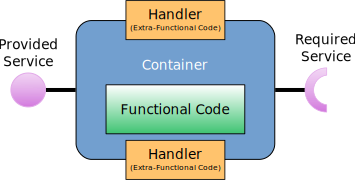
\includegraphics[width=\textwidth]{../imgs/cbse_component}
\end{frame}

\begin{frame}{Component Life Cycle}
\centering

\tikzset{
    %Define standard arrow tip
    >=stealth',
    %Define style for boxes
    punkt/.style={
           rectangle,
           rounded corners,
           draw=black, very thick,
           fill=yellow!30,
           text width=7em,
           minimum height=2em,
           text centered},
    % Define arrow style
    pil/.style={
           ->,
           thick,
           shorten <=2pt,
           shorten >=2pt,}
}

\begin{tikzpicture}[node distance=2.5em, auto]
\node[circle, draw, very thick, fill=yellow!30] (init) {};
\node[punkt, below=of init] (instantiated) {INSTANTIATED};
\node[punkt, right=10em of init] (validating) {VALIDATING};
\node[punkt, below=of validating] (valid) {VALID};
\node[punkt, below=of valid] (invalidating) {INVALIDATING};
\node[punkt, below=of instantiated] (deleted) {DELETED};
\node[circle, draw, very thick, fill=black, below=of deleted] (final) {};

\draw[pil] (init.south) to node[auto, swap] {Instantiate} (instantiated.north);
\draw[pil] (instantiated.east) to node[auto] {Validate} (validating.west);
\draw[pil] (validating.south) to node[auto] {} (valid.north);
\draw[pil] (valid.south) to node[auto] {Invalidate} (invalidating.north);
\draw[pil] (invalidating.west) to node[auto] {} (instantiated.east);
\draw[pil] (instantiated.south) to node[auto, swap] {Remove} (deleted.north);
\draw[pil] (deleted.south) to node[auto] {} (final.north);
\end{tikzpicture}
\end{frame}

\subsection{Code Snippets}

\begin{frame}[fragile]{Snippet: Sample Component}
\begin{block}{Hello world sample}
\begin{minted}{java}
@Component(name="my-factory"}
@Provides(specification=MyInterface.class)
@Instantiate(name="my-instance")
public class MyImplementation implements MyInterface {

	@Requires(optional=true)
	private LogService logger;
	
	public void hello(String name) {
		System.out.println("Hello, " + name + "!");
		logger.log(LogService.LOG_DEBUG,
			"Said hello to " + name);
	}
}
\end{minted}
\end{block}
\end{frame}
